%
% LaTeX template for prepartion of submissions to PLDI'15
%
% Requires temporary version of sigplanconf style file provided on
% PLDI'15 web site.
% 
\documentclass[pldi]{sigplanconf-pldi15}

\usepackage{graphics}
\usepackage[pdftex]{graphicx}% Include figure files
\usepackage{bm}
\usepackage{natbib} % necessary for bibtex
\usepackage[toc,page]{appendix}
\usepackage{pgffor}
\usepackage{minted}
\usepackage{syntax}

%
% the following standard packages may be helpful, but are not required
%
\usepackage{SIunits}            % typset units correctly
\usepackage{courier}            % standard fixed width font
\usepackage[scaled]{helvet} % see www.ctan.org/get/macros/latex/required/psnfss/psnfss2e.pdf
\usepackage{url}                  % format URLs
\usepackage{listings}          % format code
\usepackage{enumitem}      % adjust spacing in enums
\usepackage[colorlinks=true,allcolors=blue,breaklinks,draft=false]{hyperref}   % hyperlinks, including DOIs and URLs in bibliography
% known bug: http://tex.stackexchange.com/questions/1522/pdfendlink-ended-up-in-different-nesting-level-than-pdfstartlink
\newcommand{\doi}[1]{doi:~\href{http://dx.doi.org/#1}{\Hurl{#1}}}   % print a hyperlinked DOI

% Grammar formatting
\setlength{\grammarparsep}{4pt plus 1pt minus 1pt}
\setlength{\grammarindent}{30em}

% minted haskell
\newmintinline{haskell}

\begin{document}

%
% any author declaration will be ignored  when using 'plid' option (for double blind review)
%

\title{DeckBuild: A Declarative Domain-Specific Language for Card Game Design}

\date{
  Matthew Ahrens, Raoul Veroy, and Karl Cronburg\\
  \texttt{\{mahrens,rveroy,karl\}@cs.tufts.edu}\\
  Dept. of Computer Science, Tufts University, Medford MA 02155\\
}

\maketitle
\begin{abstract}
\end{abstract}


% This is a possible breakdown of sections. Feel free to re-arrange / rename
% things, but try to at least keep the labels (I reference 'sec:intro'
% and 'sec:goals' later in the paper)

\section{Introduction - Target Domain \& Users} \label{sec:intro}
\subsection{Domain}
Like most table top or board games, deck building card games do not have many automated systems or
testing tools for their general use or creation. Only the most popular games in the genre have software that
either simulates playing it or running strategies. Typically the software is closed or propritary, and
making changes to the software to fit personal needs or a new game is discourged. We have identified a need
to facilitate the creation and testing of new deck building card games.
\subsection{Users}
The intended audience for DeckBuild is card game makers who want
an easy way to describe and test new cards, card types, or card game rules. Specifically, DeckBuild
supports describing cards and rules from the subgenre of deck building card games such as Dominion or Magic the
Gathering. The card game makers we are expecting who will adopt DeckBuild either have a programming
background or will be working closely with a programmer.
\\
In its current iteration, the DeckBuild
suite provides an easy way to represent cards that can be consumed in other parts via the runtime system
library. The technical maker or programming partner can then connect the functionality of the cards to
the runtime library in any way they wish and use provided artifacts such as a game client to test the cards
or AI with custom heuristics. While we hope to make those tools work without manipulating the
runtime library behind the scenes to lower the barrier of entry to our language, if the card game maker
wishes to assess new functionality in their cards and game rules through these artifacts, then
they should be prepared to provide some implementation of their own. Card game makers who wish to
extend only the gammar of existing poplar deck building games will find all that functionality
come free with DeckBuild.
\subsection{Existing Languages}
There are currently no languages suited to describing features of deck building card games in general
terms. There exists software such as Dominion Online or Magic the Gathering Online which exists as
a way to play those offical titles with people or against AI.
The closest competitor for DeckBuild is Dominiate, an
open source project by Robert Speer that is a Dominion Simulator written in coffeescript.
\\
Dominiate provides a way for end users to specify policies for Dominion AI in terms of:
what priority to buy cards in, what priority to play cards in, and other heuristics available
to the player at any game state. While DeckBuild and Dominiate share a common goal of letting users evaluate
strategies of given combinations of cards, Dominiate does not give support for arbitrary or new cards.
Logic for cards and rules is distributed across its runtime system making it
difficult to add functionality for new cards. Dominiate can then be seen not as a language competitor
 for game makers to compare, but rather a runtime system that DeckBuild would hope to leverage in the
 future as an output format. Specifially, it would benefit both communities to be able to specify
 cards and rules in DeckBuild, but output cofeescript source for use in the Dominiate simulator.
\section{Goals} \label{sec:goals}
DeckBuild is at its core a way for card game makers to describe cards and provide that description
for use in general purpose programs or tools. Our goals reflect that and are more end user centered than
performance or optimization focused.
\subsection{Readability}
Currently two representations for Deck Building cards are accepted by the communities. The game maker
community represents the card as a physical artifact with plain english functional descriptions
of what the card can do. This is very ambiguous and difficult to parse. The
programmer making tools for these games represents cards as the functionality and utility of how the
card affects the game state. While concrete, this representation is hard to collect and can be difficult to read
if written across a system in general purpose programming code. We aim to compromise
on making a card and rule representation that can be used functionally within a program, but maintains
the human readability that it would have as a physical artifact.
\subsection{Consumability}
In implementation, programmers usually describe cards and rules by how that specific card affects the game
state. This means that the use of each card and what each card requires can be widely different, with the burden
of guaranteeing functional saftey on the programmer. If a new card requires a specific resource of the game
state or runtime, it should be obvious upon describing the card. This could be done through Object Oriented like interfaces or other contractual classification
of card objects, but that can quickly become difficult to manage, especially for a large number of cards. We hypothesize that
by representing cards and rules in a uniform syntax and parsing them in Haskell, we can easily provide type saftey and
card requirements to any runtime system that wants to consume our representation.
\subsection{Support and Resources}
The DeckBuild Language can better benefit its early adopters if they have fun tools to play with out-of-the-box to test their new cards and game rules against.
We hope to achieve, for the programmers working
with these card game makers, an easy way to take the standard game representations and integrate it in their
programs. We overcome their initial hurdle by providing a game state system runtime with AI and client interfaces
that consumes cards and provides a framework for specifying new functionality in Haskell. Eventually, it would fully
realize our goal if the programmer could provide the functionality that corresponded to abstract representation of arbitrary
english card descriptions that DeckBuild parses, and then the language automatically makes those connections. For example, if a new
simulator were to be released that takes card representations in a novel way, the programmer should be able to simply write the artifact
generator from our Abstract Representation to that new format. This way the both the programmer and the card game maker gain the benefit
of interoperability and support.
\subsection{Metrics and Measurement}
Since the goals of DeckBuild are people centric, the successfulness of our language can be measured as the quantified
amount of effort it takes for the programmer to connect the output of the defined cards and rules to the runtime implementation of their
choice. Reducing this effort can come about from meeting any of the goals formerly described. Making the code readable, yet unambiguous
lets the programmer reuse functionality since the size of the grammar they must support is smaller. Making the internal representation of
the card type safe and consumable reduces the amount of checks the programmer must perform before trying to integrate the functionality of
the card with a new system. Lastly, through good tool support and out-of-the-box functionality, we hope to abstract away most of the common
boiler plate the programmer would want to write such as a generic card game simulator or client-server system.
\\
For this initial implementation, we also measure the effectiveness in terms of the expressiveness that the card game author gets
without having to imploy their programmer or technical side. We can show this completeness by being able to describe any arbitrary cards from the
official Dominion set. We hope to show that these aspects of our language are complete while still remaining robust enough to describe any
new card. The observable metric of how robust our language is can be then seen as how well we minimize the amount of code the programmer has to
write in using our runtime library when providing functionality for these new cards.


\section{Language Features}
\label{sec:features}
% 5. Describe the features your language provides and explain why this set of
% features is appropriate.
The current iteration of DeckBuild gives a game designer the
following features:

\begin{itemize}
\item Declarative enumeration of the content of a card comprising its
      \emph{name}, card \emph{type},
      what the card does when played (\emph{effects}), and the \emph{cost}
      of the card in order to buy it.
\item Declarative enumeration of the parameters to the mechanics of a turn in
      the game, namely the number
      of \emph{actions} and \emph{buys} a player starts with on each turn,
      the number of cards \emph{discarded} at the end of a turn, and the
      number of cards \emph{drawn} in-between turns.
\end{itemize}

These features give game designers a way to quickly express new cards and
game mechanics. This speed of prototyping new deckbuilding game variants
facilitates the exploration process. Namely, a deckbuilding game designer
will likely have a general idea what the cards should do, and have a
feeling that they will interact well together. Coming up with specific
numbers to put on the cards however requires \emph{exploring} the state
space of possible cards.

This process is indicative of what DeckBuild should give a game designer.
Although this set of features leaves much to be desired (see Section
\ref{sec:future} for full discussion), we believe it to be appropriate
for our goals.

See the last appendix for a complete grammar for DeckBuild.

% TODO: figure out how to get RHS grammar indenting to work properly...
%\subsection{Grammar}
%\begin{footnotesize}
%\begin{grammar}
%% -----------------------------------------------------------------------------
% - Top-level decls:

<deckDecls>  ::= <deckDecl>*

<deckDecl>   ::= <cardDecl> | <turnDecl>

% -----------------------------------------------------------------------------
% - Card declaration grammar rules:

<cardDecl>    ::= "card" <cardID> "::" <cardType> "{" <cardDescr> "}" "costs" <intLit>

<cardDescr>   ::= <effectDescr>* <englishDescr>

<englishDescr> ::= <stringLit>*

<effectDescr>  ::= <plusOrMinus><intLit> <effectType>

<plusOrMinus> ::= "+" | "-" 

% -----------------------------------------------------------------------------
% - Phase / rulebook declaration grammar rules:
% -   TODO: custom named phases (future), rulebook for custom rules other than turns

<turnDecl>   ::= "turn" <turnID> "{" <phaseDescr>* "}" 

<phaseDescr> ::= <phaseName> <phaseInt>

<phaseInt>   ::= <intLit> | "all"

% looks like: phases {Action 1 Buy 1 Discard all Draw 5} for standard rules.

% -----------------------------------------------------------------------------
% - Keyword and built-in-to-parsec grammar rules:
<effectType>  ::= "actions"   | "coins"  | "buys" | "cards" | "victory"

<cardType>    ::= "Treasure" | "Action" | "Victory"

<phaseName>   ::= "action"   | "buy"    | "discard" | "draw"

<*ID>         ::= <identifier>

<*Lit>      ::= As defined in Text.Parsec.Token

<identifier>  ::= As defined in Text.Parsec.Token

% Note that we don't actually need to specify the type as that is implied by the
% action
% Maybe add these back? Not sure if we need these. - Raoul
%
% <charLit>    ::= As defined in Text.Parsec.Token
%
% <stringLit>  ::= As defined in Text.Parsec.Token
%
% <identifier> ::= As defined in Text.Parsec.Token
%
% <whiteSpace> ::= As defined in Text.Parsec.Token

%\end{grammar}
%\end{footnotesize}

\subsection{Example Program}
% 6. Show at least one sample program in your language and explain what it
% does.

\inputminted
[ %frame=lines
, framesep=2mm
, fontsize=\footnotesize %\small %\tiny
%, linenos
] {haskell}{BaseQuote.hs}

Above is a complete example program. The program defines ten cards and
one turn mechanics declaration. The ten cards are parsed and then compiled
into a Haskell function \mintinline{haskell}{kingdomCards :: [RuntimeCard]}.
The ten cards are also parsed into an enumeration data type where,
for example, \mintinline{haskell}{VILLAGE :: CardName}. This in particular
facilitates the use of host-language features of Haskell when designing
cards with decidedly non-declarative effects (see
Appendix \ref{appendix:complexcard} ) for an example).
The turn declarations are parsed and compiled in the same manner as the
card declarations, except they are compiled into a Haskell function
\mintinline{haskell}{turnRules :: [Turn]}.

% 7. Describe how you implemented the language.
The compilation just described is performed using Haskell's quasiquotation
facilities. As a result, the recommended programming pattern is to define
a single \mintinline{haskell}{[deck| ... |]} quasiquoted program at the
beginning of a Haskell module. The Haskell module is named based on why the cards in
the module are being group together. For example, a deckbuilding game based
on World War II might have a module named `WWII' containing cards named
after airplanes used in World War II.

With a complete deck of cards defined in a module, the runtime system now
consumes said module. Presently the runtime system can be interfaced with
in three ways:

\begin{itemize}
\item As a Haskell backend API for performing probabilistic inference
      on the possible states of the game given a model for the play
      heuristics of two computer-players playing the game. This is where
      the Machine Learning users (with Haskell experience) interested
      in deckbuilding games can use DeckBuild.
\item As a web socket API for designing web-based deckbuilding games.
      This is where web programmers (with minimal to no Haskell experience)
      can make use of DeckBuild to create a deck build game and corresponding
      web site tailored to their genre of interest.
\item As a command-line interface for humans to play against one another
      (making use of the web sockets API). This is where a game designer can
      have human subjects play-test their game without having to print out
      mock-ups of cards.
\end{itemize}

% 8. Explain what if any services are provided in a “run-time system.”
The runtime system itself is implemented as a Haskell cabal package separate
from (but referencing / importing) the DeckBuild language package. It is
implemented in the state monad for maintaining a stateful view of the game
as turns progress. We also use the IO monad for executing
player-based events in the game. The core components of the runtime system
handle functionality common to all deckbuilding games comprising:

\begin{itemize}
\item Maintaining piles of cards
  \begin{itemize}
  \item Moving cards between decks (enforcing no `card-duplication-bugs')
  \item 
  \end{itemize}
\item Library of:
  \begin{itemize}
  \item Getters and setters for \mintinline{haskell}{Game} state
  \item Execution of common events:
    \begin{itemize}
    \item \mintinline{haskell}{draw     :: State Game ()}
    \item \mintinline{haskell}{shuffle  :: State Game ()}
    \item \mintinline{haskell}{discard  :: State Game ()}
    \item \mintinline{haskell}{doPhase  :: State Game ()}
    \item \mintinline{haskell}{takeTurn :: State Game ()}
    \item \mintinline{haskell}{runGame  :: State Game ()}
    \end{itemize}
  \item Common \mintinline{haskell}{Game} state questions:
    \begin{itemize}
    \item How many cards of type `X' are in my hand?
    \item Can I currently buy card `Y'?
    \item Can I currently play card `Z'?
    \item Has the game ended? If so, who won?
    \end{itemize}
  \end{itemize}
\end{itemize}

The use of Haskell as the host-language of DeckBuild gave the runtime system
a lot of power in being able to make guarantees about the state of a game.
In particular the first-class nature of IO lets the runtime system divide
up the portions of the system which are and are not allowed to perform IO.
This division makes IO bugs impossible to create when designing and writing
purely functional components of the runtime system. Similarly, the immutable
nature of Haskell data instances makes shared-memory bugs impossible. This is
important in DeckBuild's runtime system when communication occurs between the
core components of the runtime system (functions inside the state monad)
and the computer-player \& web socket components (and other components not
allowed to directly alter the state of the game).

In the current iteration of our language and the runtime system, certain
concepts such as \mintinline{haskell}{ACTIONS} and \mintinline{haskell}{COINS}
are hard-coded into the runtime system and as concrete syntax in the language.
These names are not inherently common to all deckbuilding games, and will be
abstracted out in a future iteration of the DeckBuild language. See Section
\ref{sec:future} for a discussion of how this and other parts of the runtime
system and language will be given better abstractions in the future.



\begin{frame} \frametitle{Evaluation}
\begin{itemize}
\item Ease of use to describe all existing dominion cards
\item Time to program the equivalent cards in other data Languages: XML, JSON, YAML
\item In next iteration, when able to express card effects
  \being{itemize}
  \item How english-like expressing difficult card effects is
  \item How complex the card effects can be
  \item How intuitive it is to do both at the same time
  \end{itemize}
\end{itemize}
\end{frame}


\begin{frame} \frametitle{Future - Tool Support}
\begin{itemize}
\begin{small}
\item Type-checker
\item Debugging information
%  \begin{itemize}
%  \item Line numbers
%  \item Common programming mistakes
%  \item Mis-spellings (e.g. `Did you mean ...?`)
%  \end{itemize}
\item Automated card \emph{balancer} (e.g. `Maybe card XXX should be \$1 cheaper.`)
\item Develop more complex card examples for reference use
\item Library of AI players using various heuristics
\item Markup language conversion tools / support
\item Graphical (in-browser flash game?) client-server support
\end{small}
\end{itemize}
  \begin{center}
    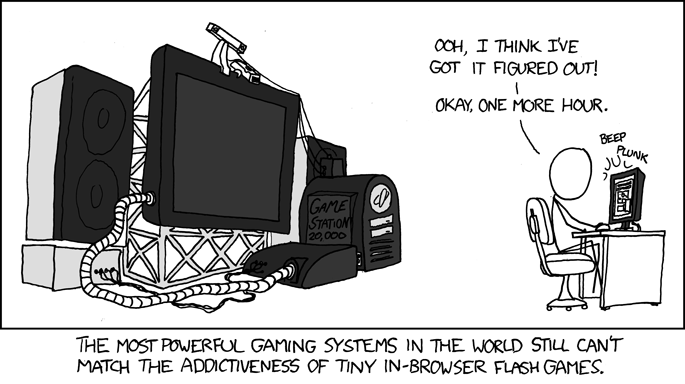
\includegraphics[width=.5\columnwidth]{flash_games.png}
  \end{center}
\end{frame}

\begin{frame} \frametitle{Future - Language Goals}
\begin{itemize}
\item Language support for English-like effect descriptions
\item Card-balancing algorithm
\item Comma-delimited syntactic sugar
\end{itemize}
\end{frame}



% We recommend that you use BibTeX.  The inlined bibitems below are
% used to keep this template to a single file.
{\softraggedright
\bibliographystyle{abbrvnat}
\bibliography{deckbuild}
}

%\begin{thebibliography}{}
%\end{thebibliography}

%\onecolumngrid
\clearpage
\onecolumn
\appendix

\section{Example Program - Haskell Output}
\inputminted
[ frame=lines
, fontsize=\small %\fontsize{1mm}{1mm} %\tiny
, framesep=2mm
%, linenos
] {haskell}{../pres/QuoteOutput.hs}

\section{Example Program - Complex Card Effects}

\inputminted
[ frame=lines
, framesep=2mm
, fontsize=\small %\fontsize{1mm}{1mm} %\tiny
, linenos
] {haskell}{../pres/ComplexEffects.hs}

The code above defines the state transformation to be performed on the game when
a \mintinline{haskell}{CELLAR} is played. The state monad is required because
the effect moves cards around between piles in the state of the game. The IO monad
is also required because the \mintinline{haskell}{CELLAR} effect requires asking
the player to pick cards. This example also illustrates the use of:
\begin{itemize}
\item \mintinline{haskell}{cards   :: Pile   -> [CardName]}, 
\item \mintinline{haskell}{hand    :: Player -> Pile}
\item \mintinline{haskell}{p1      :: Game   -> Player}
\item \mintinline{haskell}{mayPick :: Game   -> CardName -> IO (Maybe CardName)}
\end{itemize}
These are the kinds of operations DeckBuild will support natively in the
future when it has support for function declarations and expressions.

\section{Runtime System - State Format}
\begin{small}
$\lambda$\verb|> runGreedy (0.5, 0.5)|
\end{small}
\begin{Verbatim}[fontsize=\small]
Player1:
    name   = "Greedy1"
    hand   = [ESTATE, GOLD, PROVINCE, PROVINCE, SILVER]
    inPlay = []
    deck   = [SILVER,   PROVINCE, COPPER, SILVER,  COPPER
             ,ESTATE,   COPPER,   COPPER, VILLAGE, VILLAGE
             ,PROVINCE, ESTATE,   SILVER, COPPER]
    dscrd  = [SILVER, SILVER, SILVER, COPPER, COPPER, PROVINCE]
    buys=1, actions=1, money=0

Player2:
    name   = "Greedy2"
    hand   = [COPPER, COPPER, COPPER, COPPER, VILLAGE]
    inPlay = []
    deck   = [SILVER,   SILVER, GOLD, COPPER, COPPER,   ESTATE
             ,GOLD,     ESTATE, GOLD, ESTATE, PROVINCE, VILLAGE
             ,PROVINCE, GOLD]
    dscrd  = [SILVER, COPPER, SILVER, SILVER, SILVER, PROVINCE]
    buys=1, actions=1, money=0

Trash: []
Supply: [(COPPER,60),  (CELLAR,10),  (MOAT,10),       (ESTATE,8)
        ,(SILVER,27),  (VILLAGE,6),  (WOODCUTTER,10), (WORKSHOP,10)
        ,(MILITIA,10), (REMODEL,10), (SMITHY,10),     (MARKET,10)
        ,(MINE,10),    (DUCHY,8),    (GOLD,25),       (PROVINCE,0)]
Turn #: 30
\end{Verbatim}

Above is a snapshot of the state of the runtime system after two
probabilistic computer-player models played a game against each other.
The player models are given direct access to this game-state information
on each turn of the game. In future iterations of the runtime system
their will likely be a feature whereby the players can `remember' what
they did on previous turns.

In the snapshot, the \mintinline{haskell}{Supply :: [(CardName,Int)]} where
the \mintinline{haskell}{Int} corresponds to the number of copies of
that particular card in the supply. The runtime system is implemented in
this manner so as to reduce the space-complexity constant. In a future
iteration of the runtime system, game designers will be
able to turn on and off these kinds of optimizations on a
per-\mintinline{haskell}{Pile} basis.

Similarly, a game designer may wish to specify the order in which cards
appear in a \mintinline{haskell}{Pile}. In the current implementation
of the runtime system, ordering of most piles defaults to LIFO queue
order (except a player's hand which is shown alphabetically).



\end{document}
